\documentclass[border=10pt]{standalone}
\usepackage{tikz}

\begin{document}
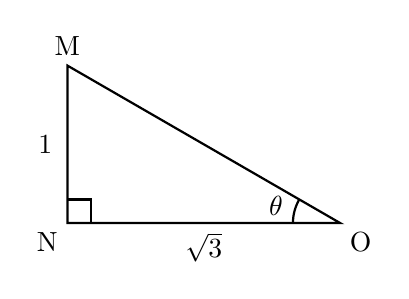
\begin{tikzpicture}[scale=1]

    % Define the vertices of the right-angled triangle
    % N is the right angle, M is the top vertex, O is the right vertex
    % Proportions: Height MN = 2, Base NO = 2 * sqrt(3) ≈ 3.464
    \coordinate (N) at (0,0);
    \coordinate (O) at (3.464,0); 
    \coordinate (M) at (0,2); 

    % Draw the triangle sides
    \draw[thick] (M) -- (N) -- (O) -- cycle;

    % Draw the right-angle symbol at N
    \draw[thick] (0.3,0) -- (0.3,0.3) -- (0,0.3);

    % Draw the angle arc at O (angle is exactly 30 degrees)
    % The arc starts at (O) and goes from 180 degrees to 150 degrees
    \draw[thick] (2.864,0) arc (180:150:0.6);

    % Add the labels for the vertices
    \node[above] at (M) {M};
    \node[below left] at (N) {N};
    \node[below right] at (O) {O};

    % Add the angle label theta
    \node at (2.65, 0.22) {$\theta$};

    % Add the side length measurements
    % "1" on the vertical side and "root 3" on the horizontal side
    \node[left, xshift=-2pt] at (0,1) {$1$};
    \node[below] at (1.732,0) {$\sqrt{3}$};

\end{tikzpicture}
\end{document}